\chapter{Amplificadores clase B y AB}


\section{Introducción}

\hspace{10pt} Las etapas de salida en clase A (en las que el dispositivo activo de
salida conduce todo el tiempo) producen una gran disipación de
potencia, inclusive en el caso en que no exista entrada de corriente
alterna. En muchas aplicaciones de amplificadores de potencia, el
circuito puede estar largos períodos de tiempo en estado de espera
sin señal de entrada, o con entrada intermitente, como en el caso de
señales de voz. La potencia disipada en estos períodos es
desperdiciada, esto implica desperdicio de potencia entregada por la
fuente de alimentación (en equipos operados por baterías esto es más
crítico aún), y aumento de la disipación en los dispositivos activos
y por lo tanto aumento de la temperatura de operación de los mismos.
La potencia disipada en los dispositivos activos afecta el tamaño
físico requerido por ellos, y por lo tanto se deben utilizar
dispositivos más costosos (dispositivos discretos de mayor tamaño y
más requerimiento de área de silicio en dispositivos integrados).

Las etapas de salida en clase B mejoran este problema, al tener una
casi nula disipación de potencia si la señal de entrada es cero.
Para entregar la potencia a la salida se utilizan, al menos, dos dispositivosactivos conduciendo medio ciclo cada uno en forma alternada. El
rendimiento de las etapas de salida clase B es mayor que las de
clase A, siendo idealmente el máximo rendimiento alcanzado del $78,5
\%$.

Las principales aplicaciones de estas etapas de salida son en:
Etapas de salida de amplificadores de audio discretos e integrados y
en etapas de salida de circuitos integrados en general.


\section{Configuraciones básicas}

\hspace{10pt}  En la figura \ref{claseb1} se muestra la configuración básica
manejada por tensión de una etapa de salida en clase B. En ella se
ve que los dispositivos de salida ($Q_1$ y $Q_2$)  son transistores
complementarios, siendo éstos idealmente iguales. En el ciclo
positivo de la tensión de entrada $v_i$ el transistor $Q_1$ conduce
y el transistor $Q_2$ se mantiene cortado, produciéndose el ciclo
positivo de la tensión de salida $v_0$ . Ocurre lo inverso en el
ciclo negativo de la tensión de entrada ($Q_1$ está cortado y $Q_2$
conduciendo).

En  la figura \ref{claseb2} se traza la curva de transferencia del
circuito, en dicha curva se ve que las pendientes en las zonas de
conducción de los dispositivos activos son aproximadamente igual a
uno (esto se debe a que actúan como seguidores de emisor). También
se notan alinealidades: una para tensiones de entrada pequeñas
debido a que los transistores están polarizados al corte,
necesitando, por ejemplo el transistor $Q_1$ una tensión mayor que
$V_{BE(on)}$  para entrar en conducción y otra por la saturación de
los transistores. Es de notar que la máxima excursión simétrica está
delimitada por esta última condición.

\begin{figure}
	\centering
	
\includegraphics[width=3.5in]{figuras/claseb1.png}\\
	\caption{Etapa de salida clase B básica.}\label{claseb1}
\end{figure}

\begin{figure}
	\centering
	
\includegraphics[width=4.5in]{figuras/claseb2.png}\\
	\caption{Transferencia de la etapa de salida clase B de la
		figura \ref{claseb1}.}\label{claseb2}
\end{figure}

Otra configuración básica es la mostrada en la figura \ref{claseb3}.
En este caso, la etapa de salida es manejada por el transistor
$Q_3$, este transistor trabaja en clase A y está polarizado de modo
que su corriente de polarización $I_{CQ3}$ sea igual a $I_Q$
(corriente que entrega el generador ubicado en la parte superior del
esquema). De tal modo los transistores $Q_1$ y $Q_2$ están
polarizados al corte, y dado que éstos son complementarios e
idealmente iguales, la tensión de salida sin señal $v_i$ de alterna
es de $0V$. Idealmente esta configuración también permitiría, como
en el caso anterior, una máxima excursión de salida limitada sólo
por la saturación de los transistores de salida, aunque para lograr
esto debe asegurarse que el transistor $Q_3$ no entre en corte antes
de que se produzca la saturación  del transistor  $Q_1$  en  el
semiciclo positivo  de  la tensión  de salida.  Es decir debe
asegurarse que:

\begin{equation}
	I_Q >\frac{\displaystyle V_{CC}-V_{CE1(sat)}}{\displaystyle (\beta +1)R_L}
\end{equation}
, en el caso en que $I_Q$ sea menor que el valor anterior, la máxima
excursión de la tensión de salida estará limitada por el corte de
$Q_3$ y será: $I_Q(\beta +1)R_L$.

\begin{figure}
	\centering
	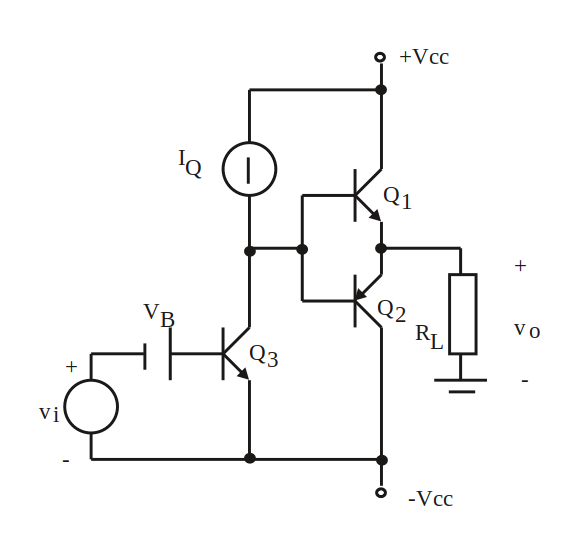
\includegraphics[width=3.5in]{figuras/claseb3.png}\\
	\caption{Etapa de salida clase B manejada por generador de corriente.}\label{claseb3}
\end{figure}

En la figura \ref{claseb4} se muestra la transferencia del circuito
de la figura \ref{claseb3}, distinguiéndose también aquí zonas
alineales similares a las de las figura \ref{claseb2}. En la figura
\ref{claseb5} se muestra la corriente de colector de $Q_3$, las
corrientes de colector de los transistores de salida y la tensión de
salida en función del tiempo. Estos gráficos temporales fueron
obtenidos por simulación, utilizando transistores de baja potencia 
con una carga de $1K$, pudiéndose observar la alternancia en la conducción entre $Q_1$ y $Q_2$ propia de los amplificadores clase B:

\begin{figure}
	\centering
	
\includegraphics[width=4.5in]{figuras/claseb4.png}\\
	\caption{Transferencia de la etapa de salida clase B de la
		figura \ref{claseb3}.}\label{claseb4}
\end{figure}

\begin{figure}
	\centering
	
\includegraphics[width=4.5in]{figuras/claseb5.png}\\
	\caption{Simulación el circuito de la figura \ref{claseb3}.}\label{claseb5}
\end{figure}

En las figuras \ref{claseb6} a) y b) se muestran etapas de salida
clase B básicas, utilizando una fuente simple. En ambos casos la
fuente de C.C. conduce la mitad del tiempo, la otra mitad del tiempo
es el capacitor $C_L$ el que entrega la energía necesaria a la
carga. La carga que entrega el capacitor en dicho ciclo es
recuperada en el ciclo siguiente, suministrada por la fuente de C.C.
El capacitor debe ser lo suficientemente grande, tal que aún para la
menor frecuencia de trabajo no disminuya considerablemente su valor
de tensión durante el semiciclo que entrega carga, en otras
palabras, debe comportarse aproximadamente como un corto circuito
frente a $R_L$ para la menor frecuencia de trabajo. Los transistores
deben estar polarizados de modo que el nodo de unión de sus emisores
esté a $\frac{\displaystyle V_{CC}}{\displaystyle 2}$, por lo tanto
la tensión de continua de $C_L$ debe ser también
$\frac{\displaystyle V_{CC}}{\displaystyle 2}$. Suponiendo
consideraciones similares a las hechas en los circuitos de las
figuras \ref{claseb1} y \ref{claseb3} para los transistores de
salida la máxima excursión de la tensión de salida será en este caso
$\simeq \frac{\displaystyle V_{CC}}{\displaystyle 2}$.

\begin{figure}
	\centering
	
\includegraphics[width=3.5in]{figuras/claseb6.png}\\
	\caption{Clase B con fuente simple. a) Manejada por tensión, b)
		manejada por corriente.}\label{claseb6}
\end{figure}



\section{Potencia de salida, rendimiento y potencia disipada en los  transistores de salida
	de una etapa clase B}

Partiendo de la configuración básica de la figura \ref{claseb1} y
suponiendo que:

\begin{itemize}
	\item  $V_o$ de C.C. es $0V$.
	\item  $Q_1$ y $Q_2$ son transistores complementarios de iguales
	características.
	\item  $V_{CE(sat)}$ de ambos transistores $\simeq 0$.
	\item  $v_i$ puede excursionar de modo de poder saturar a
	los transistores.
	\item Se desprecia la distorsión que se produce en el
	cruce por $0V$.
	\item La señal de entrada $v_i$ es senoidal.
\end{itemize}

Se puede obtener lo siguiente:

\bigskip

\textbf{Potencia de salida PL}

\medskip

La potencia de salida sobre $R_L$ es:

\begin{equation}
	P_L=\frac{\displaystyle \hat{v}_o^2}{\displaystyle 2R_L}
\end{equation}


La potencia máxima de salida (suponiendo que $v_o$ puede excursionar
$\pm V_{CC})$ es:

\begin{equation}
	P_{Lmax}=\frac{\displaystyle V_{CC}^2}{\displaystyle 2R_L}
\end{equation}

\medskip

\textbf{Potencia entregada por las fuentes de C.C.}

\bigskip

Si la corriente de colector de $Q_1$ (y de $Q_2$) tiene la forma
mostrada en la figura \ref{claseb5} (media onda senoidal), la
corriente media será:

\begin{equation}
	\bar{i}_{C1}=\bar{i}_{C2}=\frac{\displaystyle \hat{i}_{C}}{\displaystyle \pi} \simeq \frac{\displaystyle \hat{v}_{o}}{\displaystyle \pi R_L}
\end{equation}


Por lo tanto la potencia entregada por las dos fuentes de continua
será:

\begin{equation}
	P_{Alimentacion}=V_{CC}\bar{i}_{C1}+V_{CC}\bar{i}_{C2}=2V_{CC}\frac{\displaystyle \hat{v}_o}{\displaystyle \pi R_L}
\end{equation}

\medskip

\textbf{Rendimiento}

\bigskip

El rendimiento de la etapa de salida, definido como el cociente de
la potencia de alterna en la salida sobre la potencia total
entregada por las fuentes de C.C. es:

\begin{equation}
	\eta=\frac{\displaystyle P_L}{\displaystyle P_{Alimentacion}}=\frac{\displaystyle \pi \hat{v}_{o}}{\displaystyle 4 V_{CC}}
\end{equation}

El rendimiento máximo se da para el caso de máxima excursión de
salida ($\hat{v}_{o}=V_{CC}$) y es de:

\begin{equation}
	\eta_{max}=\frac{\displaystyle \pi}{\displaystyle 4}=0.7854
\end{equation}

, es decir el 78,54 \% en su versión porcentual.

\medskip

\textbf{Potencia disipada en los transistores de salida}

\bigskip

La potencia disipada en los transistores de salida se puede calcular
del siguiente modo:

\begin{equation}
	P_{D(Q_1+Q_2)}=P_{Alimentacion}-P_L
\end{equation}

\begin{equation}
	P_{D(Q_1+Q_2)}=\frac{\displaystyle 2V_{CC}\hat{v}_{o}}{\displaystyle \pi
		R_L}-\frac{\displaystyle \hat{v}_{o}^2}{\displaystyle 2R_L}
\end{equation}

La máxima potencia disipada por los transistores se obtiene
derivando dicha potencia con respecto al valor pico de la tensión de
salida e igualándola a cero.

\begin{equation}
	\frac{\displaystyle \partial P_{D(Q_1+Q_2)}}{\displaystyle \partial
		\hat{v}_{o}}=\frac{\displaystyle 2V_{CC}}{\displaystyle \pi
		R_L}-\frac{\displaystyle \hat{v}_{o}}{\displaystyle R_L}=0
\end{equation}


De aquí se obtiene que la máxima potencia disipada por los
transistores se da para el caso en que la tensión pico de salida
sea:

\begin{equation}
	\hat{v}_{o}=\frac{\displaystyle 2V_{CC}}{\displaystyle \pi}
\end{equation}


Por lo tanto la potencia disipada máxima en los dos transistores
será:

\begin{equation}
	P_{D(Q_1+Q_2)}=\frac{\displaystyle 2V_{CC}^2}{\displaystyle \pi^2 R_L }
\end{equation}


Debido a que cada transistor conduce la mitad del tiempo y a la
simetría en la respuesta en ambos transistores, la potencia disipada
máxima en cada uno de ellos será la mitad del valor previamente
calculado.

\medskip

\textbf{Potencia de salida, rendimiento y potencia disipada en los
	transistores de salida de una etapa clase B con fuente simple}

\bigskip

En el caso de fuente simple y suponiendo máxima excursión posible de
la tensión de salida $\frac{V_{CC}}{2}$, se pueden desarrollar
expresiones similares a las anteriores para la potencia de salida,
rendimiento y disipación en los transistores, éstas son:

\begin{equation}
	P_L=\frac{\displaystyle \hat{v}_o^2}{\displaystyle 2R_L}
\end{equation}

\begin{equation}
	P_{Lmax}=\frac{\displaystyle V_{CC}^2}{\displaystyle 8R_L}
\end{equation}

\begin{equation}
	P_{Alimentacion}=V_{CC}\bar{i}_{C1}=\frac{\displaystyle V_{CC}\hat{v}_o}{\displaystyle \pi R_L}
\end{equation}

\begin{equation}
	\eta=\frac{\displaystyle P_L}{\displaystyle P_{Alimentacion}}=\frac{\displaystyle \pi \hat{v}_{o}}{\displaystyle 2 V_{CC}}
\end{equation}

\begin{equation}
	\eta_{max}=\frac{\displaystyle \pi}{\displaystyle 4}\quad \quad
	(\hat{v}_{o}=V_{CC}/2)
\end{equation}

\begin{equation}
	P_{D(Q_1)max}=P_{D(Q_2)max}=\frac{\displaystyle V_{CC}^2}{\displaystyle
		4\pi^2R_L}\quad \quad (\hat{v}_{o}=V_{CC}/\pi)
\end{equation}

\medskip

\textbf{Distorsión por cruce}

\bigskip

En las figuras \ref{claseb2} y \ref{claseb4} se notan alinealidades
en las transferencias en los pasajes por 0. Esto se debe a que los
transistores están polarizados con una tensión base emisor igual a
cero, necesitando una tensión $V_{BE}=V_{BE(on)}$ para comenzar a
conducir, esta diferencia es la que produce la llamada distorsión
por cruce (ver gráfico de la tensión $v_o$ en función del tiempo en
la figura \ref{claseb5}). Para mejorar esta distorsión se polarizan
los transistores al borde de la conducción (es decir $V_{BE}\approx
V_{BE(on)}$), conduciendo éstos algo más de medio ciclo. Esta
variante en la configuración de salida es la que se denomina clase
AB. En la figura \ref{claseb7} a) se polarizan los transistores con
la tensión base emisor adecuada por medio de la caída de tensión en
la resistencia R, $V_R$ debe ser igual a $2V_{BE(on)}$. En la figura
\ref{claseb7} b) se logra el mismo objetivo mediante las caídas en
los dos diodos, esta configuración tiene la ventaja de lograr una
compensación con respecto a las variaciones de temperatura, ya que
al variar ésta, varían las tensiones base emisor y en los diodos en
forma similar, produciéndose una compensación. En la figura
\ref{claseb7} c) se reemplazan los diodos por un transistor de modo
que $V_{CE}=2V_{BE(on)}$, en este circuito también se logra una
efectiva compensación con respecto a las variaciones de $V_{BE}$ con
respecto a la temperatura.

\begin{figure}
	\centering
	
\includegraphics[width=3.5in]{figuras/claseb7.png}\\
	\caption{Tres formas de mejorar la distorsión por cruce.}\label{claseb7}
\end{figure}

\section{Realizaciones prácticas de etapas de salida clase A y AB}

El circuito de la figura \ref{claseb8} es la etapa de salida
(simplificada) del amplificador operacional 709. En reposo $V_o =
V_1 = 0V$, la corriente $I_{CQ_3} = I_Q = \frac{\displaystyle
	V_{CC}}{\displaystyle R_B} = 0,5 mA$.


\begin{figure}
	\centering
	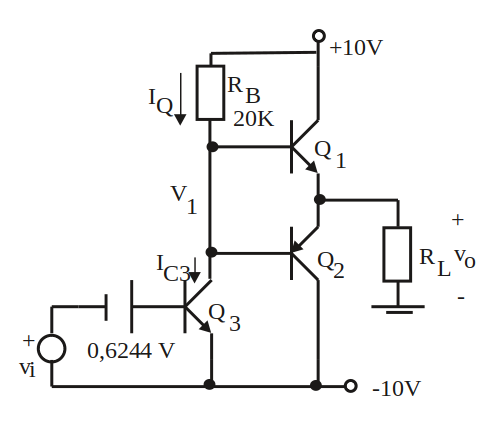
\includegraphics[width=3.5in]{figuras/claseb8.png}\\
	\caption{Etapa de salida simplificada del amplificador operacional 709.}\label{claseb8}
\end{figure}

En el semiciclo negativo de la tensión de salida $v_o$ ( semiciclo
positivo de la tensión de entrada $v_i$ y de la corriente $i_{C3}$)
el valor máximo (en valor absoluto) que puede tener $v_o$ está
determinado por la saturación de $Q_3$, es decir:

\begin{equation}
	v_{o(max)}(semiciclo-)=\mid -V_{CC}+V_{CE(sat)}+v_{EB2}\mid
\end{equation}

En este semiciclo $Q_1$ está cortado y $Q_2$ está en zona activa
actuando como un seguidor de emisor.

En el semiciclo positivo de $v_o$ ( negativo de $v_i$ y de $i_{C3}$)
$v_1$ aumenta activando $Q_1$ y cortando a $Q_2$, el límite de
excursión en este semiciclo está dado por el corte de $Q_3$. Si
$i_{C3} = 0$, entonces:

\begin{equation}
	V_{CC}=i_{B1}R_B+v_{BE1}+v_{o(max)}(semiciclo+)
\end{equation}

\begin{equation}
	v_{o(max)}(semiciclo+)=i_oR_L=(\beta_1+1)i_{B1}R_L
\end{equation}

\begin{equation}
	v_{o(max)}(semiciclo+)=\frac{\displaystyle V_{CC}-v_{BE1}}{\displaystyle 1+\frac{\displaystyle R_B}{\displaystyle R_L(\beta_1+1)}}
\end{equation}


Si $\beta_1=146$ y $R_L=10K$:

\begin{equation}
	v_{o(max)}(semiciclo+)\approx 0,986(V_{CC}-v_{BE1})
\end{equation}

Esto es del orden de $v_{o(max)}(semiciclo-)$ y cercana a $V_{CC}$.

Para el caso de $\beta_1 = 146$ y $R_L = 1K$:

\begin{equation}
	v_{o(max)}(semiciclo+)\approx 0,88(V_{CC}-v_{BE1})
\end{equation}

Aquí la excursión de la salida está determinada por el semiciclo
positivo.

En la figura \ref{claseb9} se muestra la transferencia del circuito
de la figura \ref{claseb8} obtenida por simulación, la falta de
linealidad observada se debe al reemplazo de la fuente de corriente
(ver figura \ref{claseb3}) por la resistencia $R_B$.

\begin{figure}
	\centering
	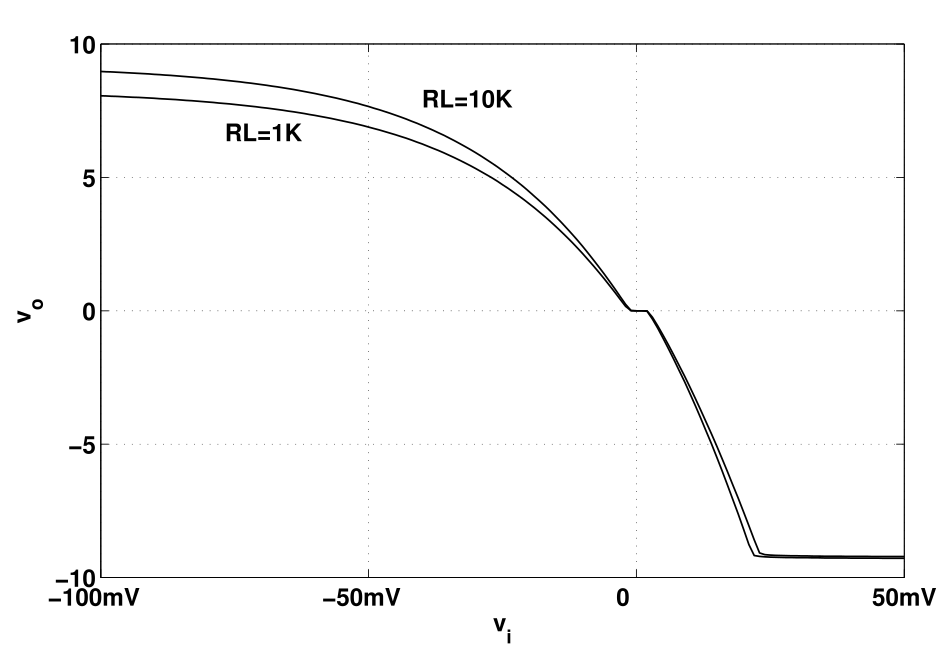
\includegraphics[width=4.5in]{figuras/claseb9.png}\\
	\caption{Transferencia del circuito de la figura \ref{claseb8}.}\label{claseb9}
\end{figure}


Para obtener una curva de transferencia con mayor linealidad se
utiliza una fuente de corriente en lugar de $R_B$, ver configuración
básica de la figura \ref{claseb3}. Una implementación práctica de
dicha configuración, puede ser la mostrada en la figura
\ref{claseb10}.


\begin{figure}
	\centering
	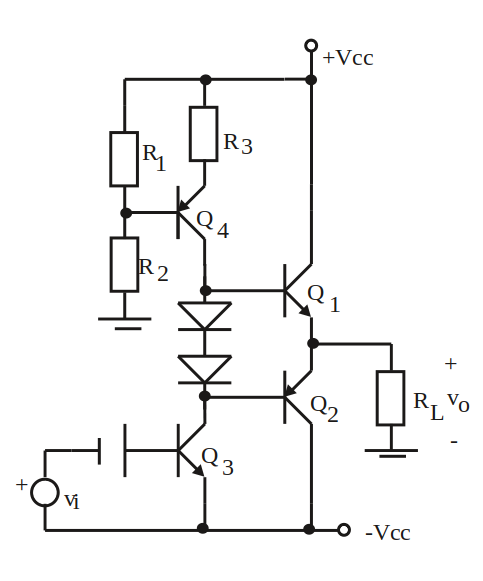
\includegraphics[width=3.5in]{figuras/claseb10.png}\\
	\caption{Etapa de salida clase AB que utiliza una fuente de corriente.}\label{claseb10} 
\end{figure}


Para este circuito debe asegurarse que $I_{CQ4}= I_{CQ3}$ y que
$Q_1$ y $Q_2$ estén cortados para $v_i = 0V$. En el semiciclo
negativo de la tensión de salida el funcionamiento es similar al
caso anterior, teniéndose también una máxima excursión de:

\begin{equation}
	v_{o(max)}(semiciclo-)=\mid -V_{CC}+V_{CE(sat)}+v_{EB2}\mid
\end{equation}

En el semiciclo positivo de la tensión de salida la máxima excursión
puede estar limitada por dos situaciones que depende del valor
elegido para $I_{CQ3} = I_{CQ4}$. Puede suceder que corte primero
$Q_3$ o que lo primero que ocurra sea la saturación de $Q_4$. Si lo
que ocurre primero es el corte de $Q_3$ ($i_{C3} = 0$), entonces:
\begin{equation}
	v_{o(max)}(semiciclo+)=I_{CQ4}(\beta_1+1)R_L
\end{equation}
, de lo contrario:
\begin{equation}
	v_{o(max)}(semiciclo+)=V_{CC}-V_{EC4(sat)}-v_{BE1}-I_{CQ4}*R_3
\end{equation}

Otra manera de implementar la fuente de corriente podría ser
utilizando una fuente ``espejo de corriente'', tal como muestra la
figura \ref{claseb11}.
\begin{figure}
	\centering
	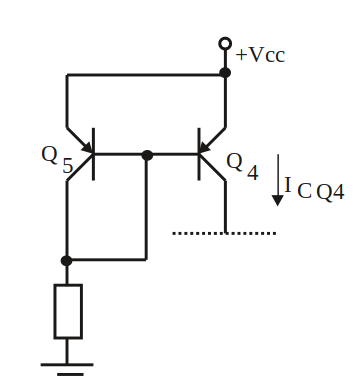
\includegraphics[width=3in]{figuras/claseb11.png}\\
	\caption{Espejo de corriente.}\label{claseb11}
\end{figure}

Aquí:
\begin{equation}
	I_{CQ4}\approx \frac{\displaystyle V_{CC}-v_{BE5}}{\displaystyle R_x}
\end{equation}
, y en el caso que sature $Q_4$ antes que corte $Q_3$, será:
\begin{equation}
	v_{o(max)}(semiciclo+)=V_{CC}-V_{EC4(sat)}-v_{BE1}
\end{equation}

En los amplificadores clase B y AB discretos, por ejemplo en la
etapa de salida de un amplificador de audio, se puede reemplazar la
fuente de corriente por un par de resistencias y un capacitor
denominado ``boostrap'' (figura \ref{claseb12}). Dicho capacitor
debe tener un valor tal que se comporte como un corto circuito, aún
para la menor frecuencia de trabajo. De tal modo que mantenga su
valor de tensión aproximadamente constante y por lo tanto se puede
decir que la tensión (y  la corriente) sobre la resistencia $R_2$
también se mantienen aproximadamente constante (se desprecia la
variación de alterna que pueda existir sobre $v_{BE1}$),
consiguiendo el ``generador de corriente'' buscado.


\begin{figure}
	\centering
	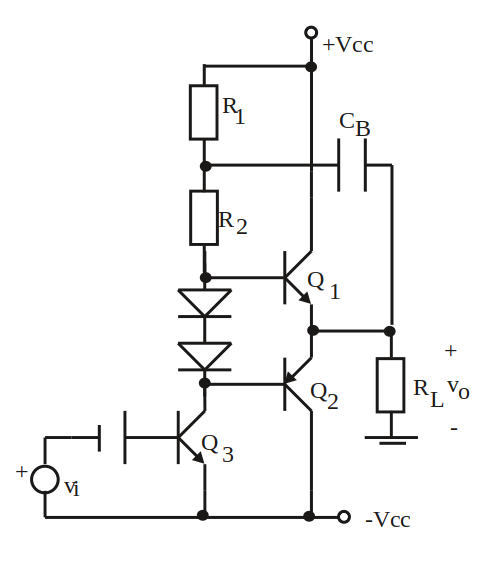
\includegraphics[width=3.5in]{figuras/claseb12.png}\\
	\caption{Circuito que incluye el capacitor de ``boostrap''.}\label{claseb12}
\end{figure}

\section{Factores térmicos que se deben tener en cuenta.}

La potencia disipada máxima en los transistores de salida (por
ejemplo $Q_1$ y $Q_2$ de la figura \ref{claseb1}) es, según lo
desarrollado anteriormente:

\begin{equation}
	P_{D(Q_1+Q_2)max} = \frac{\displaystyle 2V_{CC}^2}{\displaystyle
		\pi^2R_L}=P_{D1max}+P_{D2max}
\end{equation}

Si la etapa de salida clase B o AB está construida en forma discreta
y maneja una potencia considerable, los transistores deberán
montarse sobre disipadores para poder manejar la potencia puesta en
juego. El ``circuito'' térmico simplificado correspondiente,
suponiendo que ambos transistores se montan sobre el mismo disipador
será el mostrado en la figura \ref{claseb13}, en dicha figura
$\theta_{jc}$ y $\theta_{ca}$ son las resistencias térmicas
juntura-carcaza y carcaza-ambiente respectivamente de los
transistores $Q_1$ y $Q_2$.

\begin{figure}
	\centering
	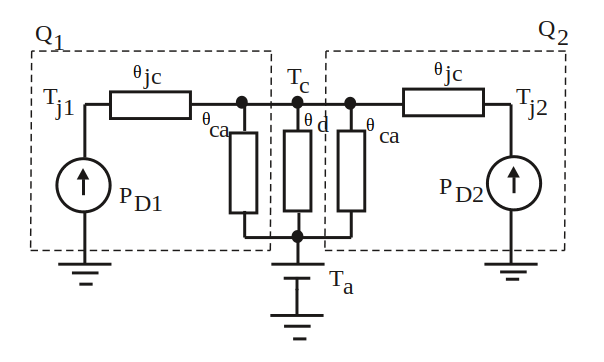
\includegraphics[width=3.5in]{figuras/claseb13.png}\\
	\caption{``Circuito'' térmico de dos transistores montados sobre el mismo disipador.}\label{claseb13}
\end{figure}

Si ambos transistores tienen características similares y suponiendo
que la resistencia térmica del disipador es:

\begin{equation}
	\theta_D \ll \frac{\displaystyle \theta_{ca}}{\displaystyle 2}
\end{equation}

Para asegurar que la temperatura de juntura de ambos transistores
sea $T_j<T_{jmax}$, se debe cumplir que:

\begin{equation}
	\theta_D < \frac{\displaystyle T_{jmax}-T_{amax}}{\displaystyle
		P_{D1max}+P_{Dmax}}- \frac{\displaystyle \theta_{jc}}{\displaystyle 2}
\end{equation}

En el cálculo anterior no se tuvo en cuenta la potencia disipada en
continua, ya que es despreciable frente a la potencia disipada en
presencia de señal de alterna. Sin embargo existe la posibilidad de
que esta pequeña potencia debida a la polarización (los transistores
de salida están polarizados muy cercanos al corte en clase AB)
produzca en fenómeno llamado enbalamiento térmico. Este fenómeno se
puede producir debido a que la corriente de colector produce
disipación en el transistor y por lo tanto aumento de temperatura,
el aumento de la temperatura produce el aumento del $\beta$ y la
disminución de la tensión $V_{BE}$, estas variaciones producen un
nuevo aumento de la corriente de colector, es decir una
realimentación positiva que puede provocar un aumento sin control de
la corriente de colector de características destructivas para el
transistor. Para que esto no ocurra debe asegurarse que la velocidad
a la que calor es generado debido a este fenómeno sea menor que la
velocidad a la que el calor pueda ser evacuado por el sistema
térmico completo (transistores más disipador). El circuito de la
figura \ref{claseb14} muestra un circuito clase AB básico sin señal
de alterna, en él la evacuación de calor está determinada por el
sistema térmico, en el cual el disipador utilizado fue dimensionado
para soportar la disipación con señal de alterna. Las resistencias
$R_E$ producen una realimentación negativa de modo de estabilizar la
corriente de colector frente a las variaciones de temperatura,
ayudando a evitar que se cumpla la condición de embalamiento
térmico.  Se mejora esto aún más cambiando la resistencia R por dos
diodos, o por un transistor (ver figuras \ref{claseb7} b) y
\ref{claseb7} c)), de modo de compensar las variaciones de $V_{BE}$
con respecto a la temperatura.

\begin{figure}
	\centering
	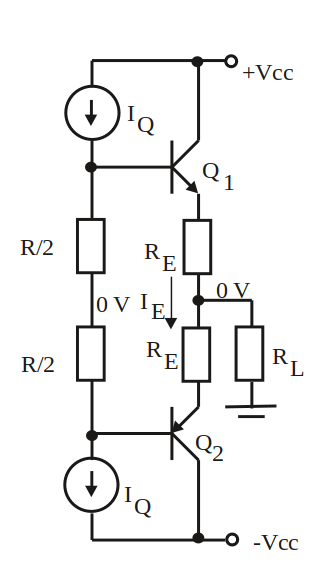
\includegraphics[width=2in]{figuras/claseb14.png}\\
	\caption{Circuito clase AB en continua.}\label{claseb14}
\end{figure}

Cuanto más grande sea la resistencia $R_E$  mejor estará
estabilizado térmicamente el circuito, sin embargo parte de la señal
de alterna caerá sobre ella por lo que se producirá una disminución
en el rendimiento, debido  a este efecto $R_E$ deberá ser lo menor
posible ($R_E = 0$ es lo mejor para la alterna). El valor óptimo
para el diseño será el menor valor de $R_E$ que asegure compensación
del efecto de embalamiento térmico. Para dimensionar $R_E$ en el
circuito de la figura \ref{claseb14} se parte de la condición de que
la velocidad a la que el calor es generado sea menor que la
velocidad a la que puede ser evacuado. De la figura \ref{claseb13}
se obtiene:
\begin{equation}
	P_{D(Q_1+Q_2)}= \frac{\displaystyle T_{j}-T_{a}}{\displaystyle \theta_{total}}
\end{equation}
; donde:
\begin{equation}
	\theta_{total}\approx \theta_d + \frac{\displaystyle \theta_{jc}}{\displaystyle 2}
\end{equation}

La evacuación del calor generado será:
\begin{equation}\label{ecuaclaseb2}
	\frac{\displaystyle \partial P_{D(Q_1+Q_2)}}{\displaystyle
		\partial T_j}=\frac{\displaystyle 1}{\displaystyle \theta_{total}}
\end{equation}

La generación del calor en la juntura estará dada por:

\begin{equation}\label{ecuaclaseb1}
	\frac{\displaystyle \partial P_{C}}{\displaystyle
		\partial T_j}=\frac{\displaystyle \partial P_{C}}{\displaystyle
		\partial I_C}\frac{\displaystyle \partial I_{C}}{\displaystyle
		\partial T_j}
\end{equation}

Donde $P_C$ e $I_C$ son la potencia disipada y la corriente de
colector de reposo de ambos transistores respectivamente. Es decir:
\begin{equation}
	P_C\approx 2V_{CEQ}I_C
\end{equation}
\begin{equation}
	\frac{\displaystyle \partial P_{C}}{\displaystyle
		\partial I_C}=2V_{CEQ}
\end{equation}
; y en este caso particular:
\begin{equation}
	\frac{\displaystyle \partial P_{C}}{\displaystyle
		\partial I_C}\approx2V_{CC}
\end{equation}

La corriente de colector del circuito de la figura \ref{claseb14}
es:
\begin{equation}
	I_C\approx I_E=\frac{\displaystyle \frac{\displaystyle I_QR}{\displaystyle 2}-V_{BE}}{\displaystyle R_E}
\end{equation}
, derivando la expresión anterior se obtiene:
\begin{equation}
	\frac{\displaystyle \partial I_{C}}{\displaystyle
		\partial T_j}=\frac{\displaystyle \partial I_{C}}{\displaystyle
		\partial V_{BE}}\frac{\displaystyle \partial V_{BE}}{\displaystyle
		\partial T_j}=-\frac{\displaystyle 1}{\displaystyle R_E} \frac{\displaystyle \partial V_{BE}}{\displaystyle
		\partial T_j}
\end{equation}

Por lo tanto según lo expresado previamente, la capacidad de
evacuación del calor (ecuación \ref{ecuaclaseb2}) debe ser mayor a
la capacidad de generarlo (ecuación \ref{ecuaclaseb1}), y teniendo
en cuenta que el coeficiente de temperatura de la tensión $V_{BE}$
es negativo se tiene que:

\begin{equation}
	\frac{\displaystyle 1}{\displaystyle
		\theta_{total}}>\frac{\displaystyle 1}{\displaystyle
		R_{E}} \left | \frac{\displaystyle \partial V_{BE}}{\displaystyle
		\partial T_j}\right |2V_{CEQ}
\end{equation}
, es decir:
\begin{equation}
	R_E>\theta_{total}\left | \frac{\displaystyle \partial V_{BE}}{\displaystyle
		\partial T_j} \right |2V_{CC}
\end{equation}

Tomándose el límite inferior de $R_E$ como valor óptimo de diseño.
Se podría colocar una $R_E$ menor si se reemplazara la resistencia R
por diodos de modo de compensar la variación de $V_{BE}$ con
respecto a la temperatura.
